\documentclass[12pt]{beamer}

% Math environment, symbols, bbm fonts, doublestroke fonts, physics for partial derivatives (pdv{}{}), breqn for multi-line equations
\usepackage{amsmath,amssymb,bbm,dsfont,physics,breqn}
% Define plim operator
\DeclareMathOperator*{\plim}{plim}
% Page size and margins
% \usepackage{geometry}
% \geometry{letterpaper,tmargin=1in,bmargin=1in,lmargin=0.75in,rmargin=0.75in}
% Line spacing
\usepackage{setspace}
\setstretch{1} % 1 for default line spacing, 2 for double, etc.
% Hyperlink environment
\usepackage{hyperref}
\hypersetup{colorlinks,linkcolor=red,urlcolor=blue,citecolor=red}
% Table environment
\usepackage{booktabs}
% Threeparttable environment
\usepackage[flushleft]{threeparttable}
% Graphic, sub-figure environments
\usepackage{graphicx, subcaption}
% Allows float options (e.g. [H] or [!ht])
\usepackage[capposition=top]{floatrow}
% Indents first paragraph
\usepackage{indentfirst}
% Footnotes go to bottom of page
\usepackage[bottom]{footmisc}
% Bibliography with AER style
\usepackage{natbib}
\bibliographystyle{aer}
% Appendix
\usepackage{appendix}

% Suppress underfull \hbox warning
\hbadness=10000

% Custom enumerate
\renewcommand{\theenumi}{\alph{enumi}}

% Result dir
\newcommand*{\FigureDir}{../graphs}
\newcommand*{\DemoDir}{../code/Rick/OUTPUT/Demographics}
\newcommand*{\SSDir}{../code/Rick/OUTPUT/SS}
\newcommand*{\TPDir}{../code/Rick/OUTPUT/TP}

% Colors
\usepackage{xcolor}
\newcommand{\red}{\color{red}}
\newcommand{\blue}{\color{blue}}

% Specify theme
\usetheme{UnofficialUChicago}

% Figures don't say "Figure" in caption
\setbeamertemplate{caption}{\raggedright\insertcaption\par}

% %%%%%%%%%%%%%%%%%%%%%%%%%%%%%%%%%%%%%%%%%%%%%%%%%
% \section{EXAMPLE USAGE OF FIGURE AND TABLE}
% %%%%%%%%%%%%%%%%%%%%%%%%%%%%%%%%%%%%%%%%%%%%%%%%%

% FIGURES

% \begin{figure}[H]
%    \centering
%    \caption{\label{fig:p\thesubsection}\autoref{sec:p\thesubsection}}
%    \scalebox{1}{
%       \begin{threeparttable}
%          \begin{tabular}{cc}
%             \includegraphics[width=0.50\textwidth]{\FigureDir/} &
%             \includegraphics[width=0.50\textwidth]{\FigureDir/} \\
%             \includegraphics[width=0.50\textwidth]{\FigureDir/} &
%             \includegraphics[width=0.50\textwidth]{\FigureDir/}
%          \end{tabular}
%       \end{threeparttable}
%    }
% \end{figure}

% SIDE BY SIDE FIGURES WITH CAPTIONS

% \begin{figure}[H]
%    \caption{\label{fig:\thesubsubsection.1}}
%    \begin{subfigure}{0.5\textwidth}
%       \centering
%       \includegraphics[width=\textwidth]{\SSDir/static/images/SS_n.png}
%       \caption{Subfig 1}
%    \end{subfigure}% <-- this "%" symbol is important
%    ~ % <-- this "~" symbol is important
%    \begin{subfigure}{0.5\textwidth}
%       \centering
%       \includegraphics[width=\textwidth]{\SSDir/dynamic_partial/images/SS_n.png}
%       \caption{Subfig 2}
%    \end{subfigure}
%    \newline <-- this creates a new lines
%    \begin{subfigure}{0.5\textwidth}
%       \centering
%       \includegraphics[width=\textwidth]{\SSDir/dynamic_full/images/SS_n.png}
%       \caption{Subfig 3}
%    \end{subfigure}%
%    ~ % <-- this "~" symbol is important
%    \begin{subfigure}{0.5\textwidth}
%       \centering
%       \includegraphics[width=\textwidth]{\SSDir/dynamic_full/images/SS_n.png}
%       \caption{Subfig 4}
%    \end{subfigure}
% \end{figure}

% TABLES

% \begin{table}[H]
%    \centering
%    \scalebox{0.75}{
%       \begin{threeparttable}\caption{\label{tab:p\thesubsection}\autoref{sec:p\thesubsection}}
%          \begin{tabular}{lcc}
%             \hline\hline\addlinespace
%             \input{../regression_tables/p1a.tex}
%             \addlinespace\hline\hline
%          \end{tabular}
%          \begin{tablenotes}
%             \item 
%             Standard errors in parentheses.
%          \end{tablenotes}
%       \end{threeparttable}
%    }
% \end{table}

% SIDE BY SIDE TABLES

% \begin{table}[H]
%    \begin{minipage}[t]{0.5\textwidth}
%      PUT TABLE 1 HERE
%    \end{minipage}% <-- this "%" symbol is important
%    \begin{minipage}[t]{0.5\textwidth}
%      PUT TABLE 2 HERE
%    \end{minipage}
% \end{table}

%\setbeamertemplate{footline}[frame number]{} % Uncomment this line if you want to remove the footer from each slide (and replace it with just the slide number (X/Y) in the bottom right of each slide.

%===============================================================%
% 				BEGIN YOUR PRESENTATION HERE					%
%===============================================================%

% Title and author information
\title[Demographic Forecasting]{\normalsize \centering Estimation Effects of Various Demographic Forecasting Techniques in Japan Using an Overlapping Generations Model}
\author{Adam A. Oppenheimer}
\institute[]{Advisor: Dr. Rick Evans\\University of Chicago}
\date{May 12, 2020}


%  \usepackage[sfmath]{kpfonts}
%  \renewcommand*\familydefault{\sfdefault}

%\setbeamerfont{frametitle}{shape=\scshape}

\AtBeginSection[]
{
    \begin{frame}
        \frametitle{Table of Contents}
        \tableofcontents[currentsection]
    \end{frame}
}

%===============================================================%
\begin{document}
%===============================================================%

\maketitle

\begin{frame}{Acknowledgements}
	I would like to thank all those who have helped me (and continue to help me) along the way to finishing my thesis. This includes Dr. Rick Evans, Dr. Kotaro Yoshida, Dr. Victor Lima, and my many friends and family who have commented on my paper (especially Kei Irizawa and Ujaan Purakayastha), among others.
\end{frame}

%===============================================================%
\section{Motivation and Research Question}
%===============================================================%

\begin{frame}{Motivation}

	\begin{table}[H]
	   \begin{minipage}[t]{0.5\textwidth}
		\begin{figure}[H]
			\centering
			\scalebox{0.8}{
				\begin{threeparttable}
					\begin{tabular}{c}
						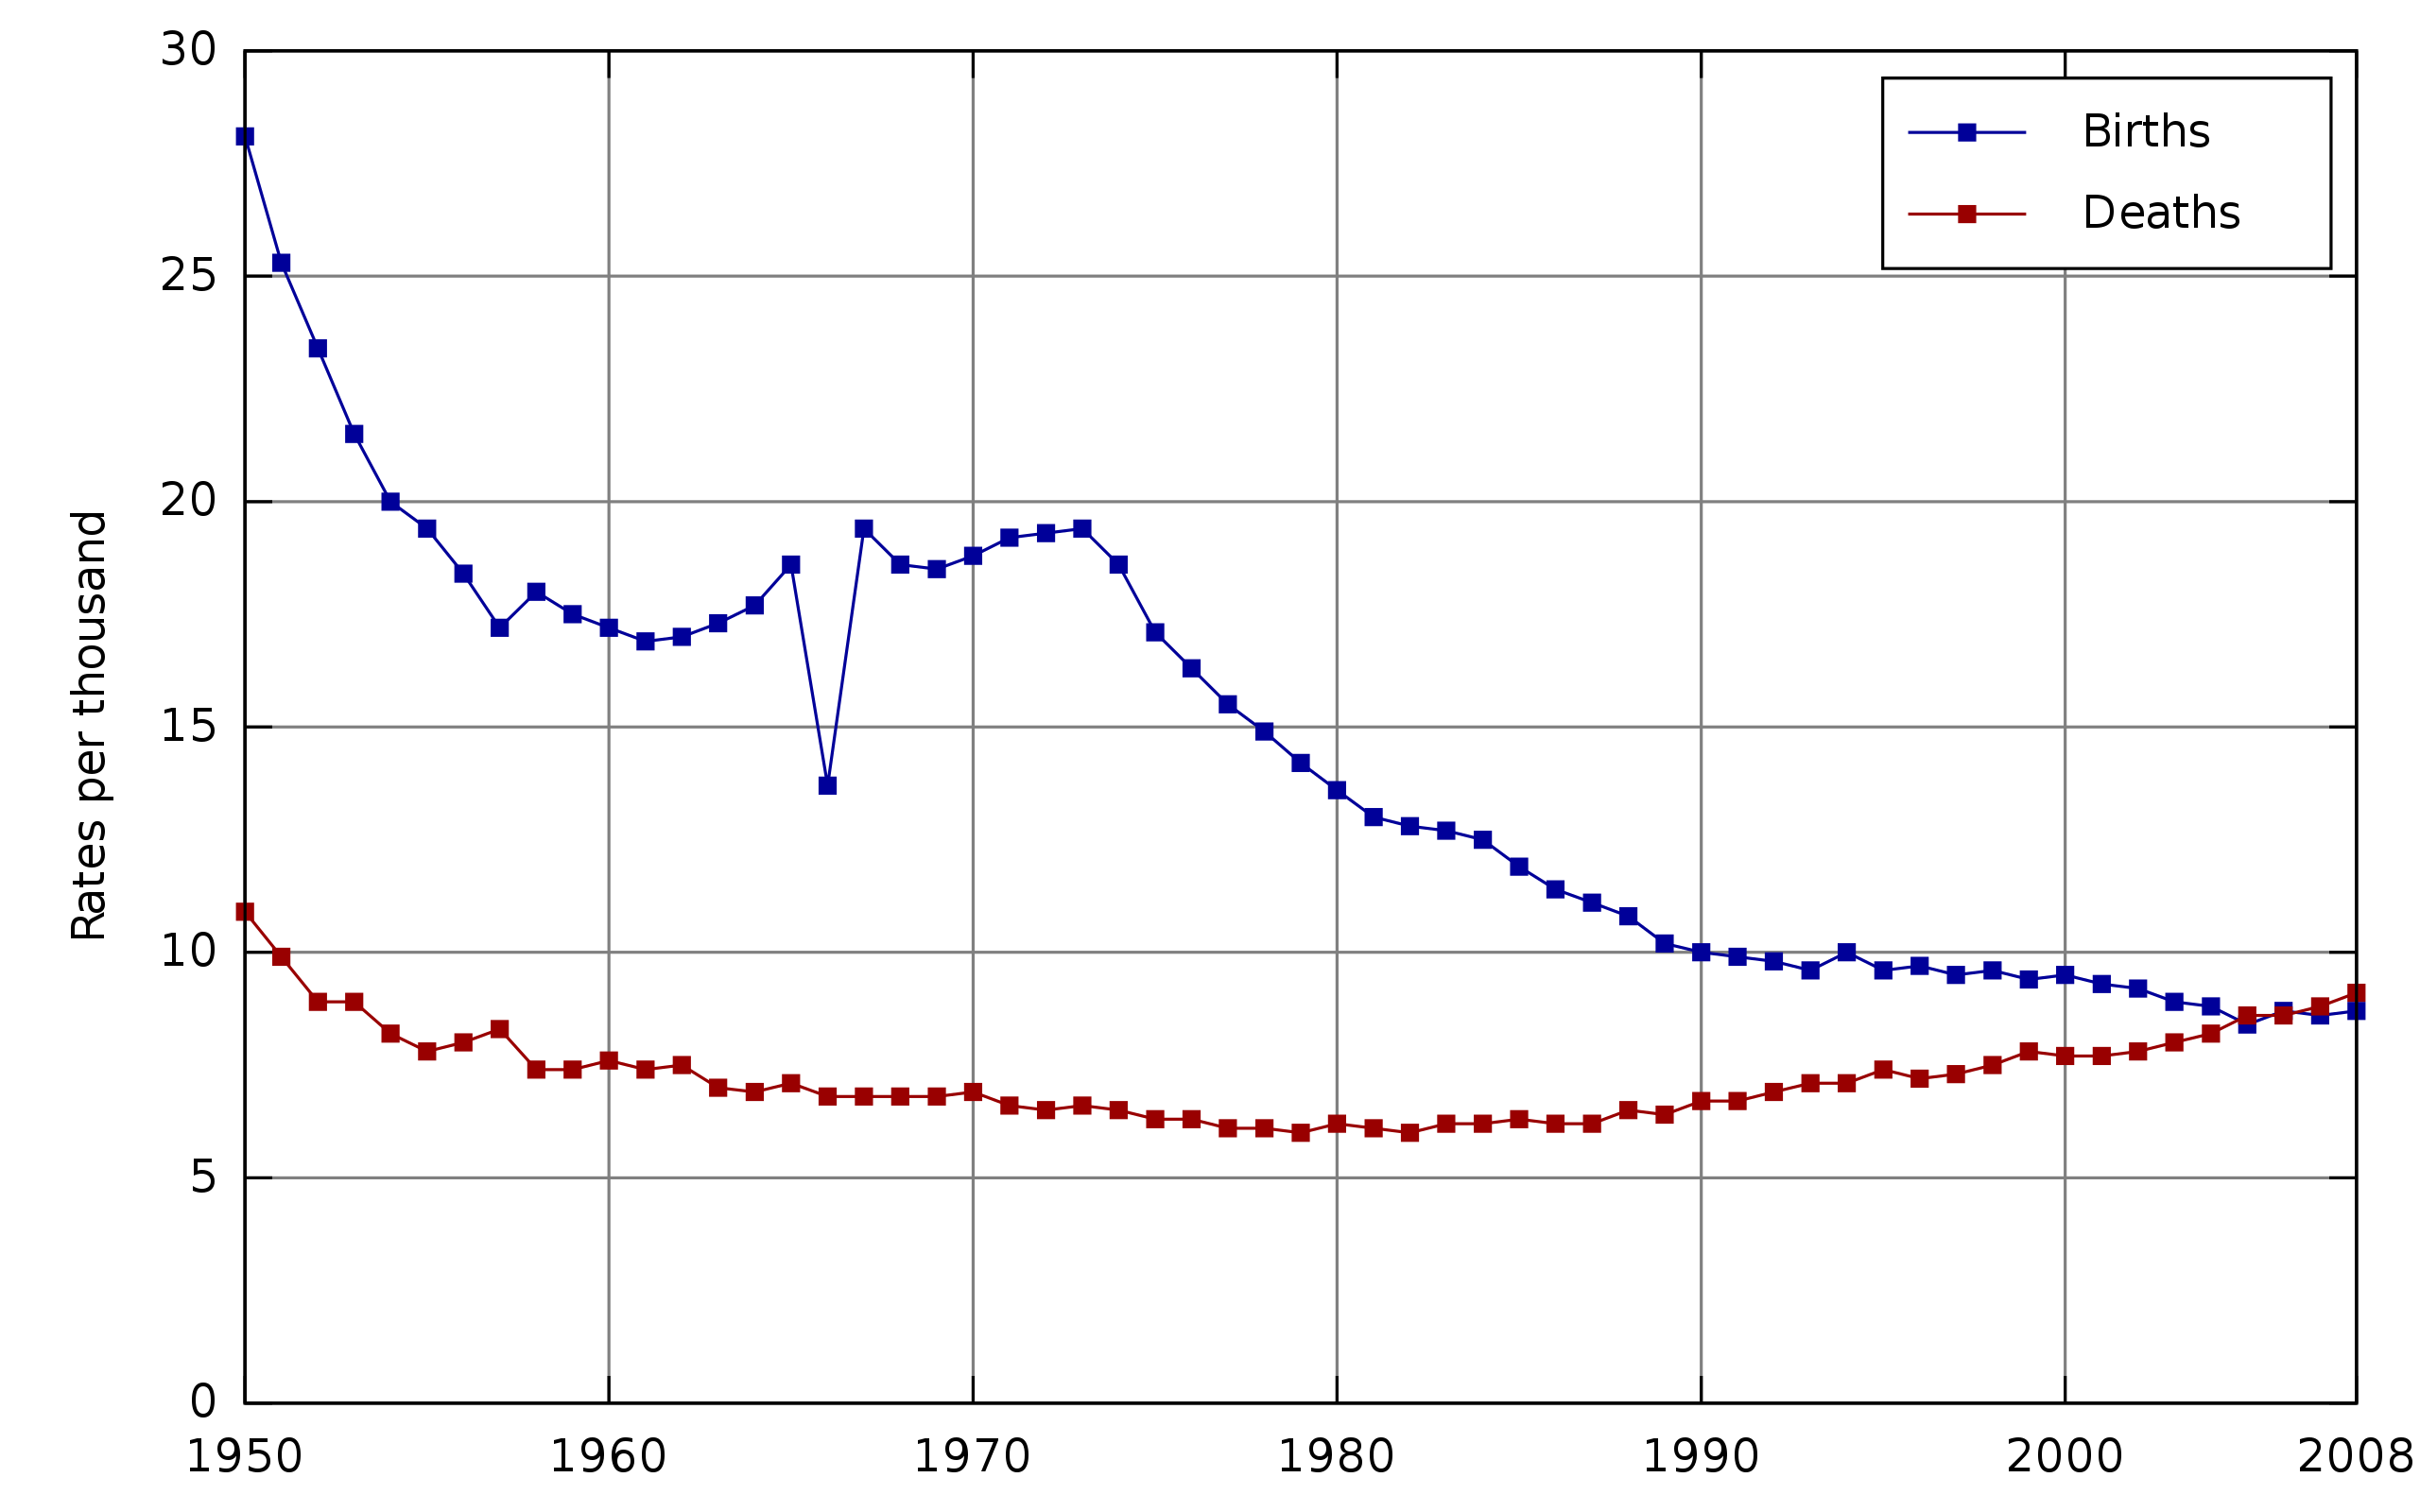
\includegraphics[width=\textwidth]{figures/birth_death_rates.png}
					\end{tabular}\vspace{-5mm}
					\begin{tablenotes}
						\item \scalebox{0.4}{Source: Wikipedia}
					\end{tablenotes}
				\end{threeparttable}
			}
			\end{figure}
	   \end{minipage}% <-- this "%" symbol is important
	   \begin{minipage}[t]{0.5\textwidth}
		\begin{figure}[H]
			\centering
			\scalebox{1}{
				\begin{threeparttable}
					\begin{tabular}{c}
						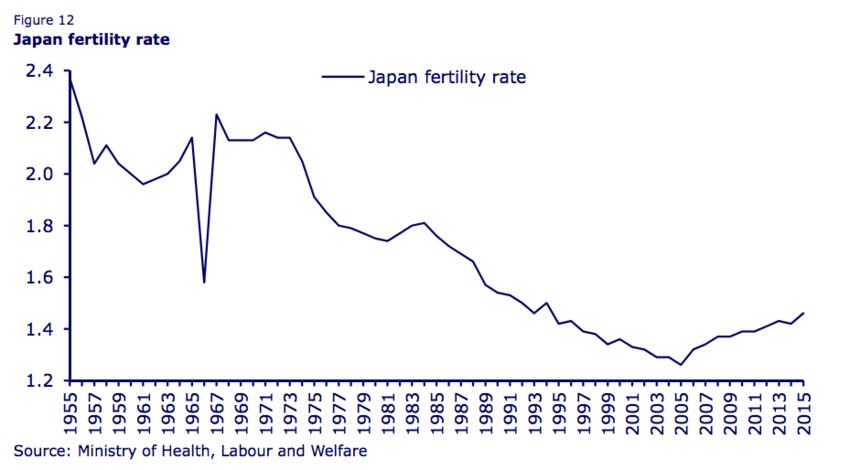
\includegraphics[width=\textwidth]{figures/fertility.png}
					\end{tabular}
				\end{threeparttable}
			}
			\end{figure}
	   \end{minipage}
	\end{table}

\end{frame}

\begin{frame}{Research Question}

	\begin{block}{Why Care?}
		What is the effect of COVID-19 mortality? How will public pensions change over time? How does predicted macroeconomic behavior respond?
	\end{block}

	\begin{alertblock}{Research Question}
		How should demographics be forecast? I propose a new method for forecasting demographics.
	\end{alertblock}

	\begin{exampleblock}{Economic Application}
		Compare macroeconomic forecasts from the most common demographic forecasting assumptions.
	\end{exampleblock}

\end{frame}

%===============================================================%
\section{Presentation Overview}
%===============================================================%
\begin{frame}{Presentation Overview}

	\begin{itemize}
		\item Data
		\item Demographic Forecasting Methods
		\begin{itemize}
			\item Static, PCA, partial dynamic, full dynamic
		\end{itemize}
		\item Macroeconomic Model
		\item Macroeconomic Results
	\end{itemize}

\end{frame}

%===============================================================%
\section{Data}
%===============================================================%
\begin{frame}{Data}

	\begin{itemize}
		\item Population and Mortality: Japanese Mortality Database (2018)
		\item Fertility: Human Fertility Collection
	\end{itemize}

\end{frame}

\begin{frame}{Population}

	\begin{figure}[H]
		\centering
		\scalebox{1}{
		   \begin{threeparttable}
			  \begin{tabular}{c}
				 \includegraphics[width=0.50\textwidth]{\FigureDir/population/smooth_0/_aggregate_true.png}
			  \end{tabular}
		   \end{threeparttable}
		}\vspace{-3mm}
		\\ \scalebox{0.7}{Population, 1970-2014}
	 \end{figure}

\end{frame}

\begin{frame}{Mortality}

	\begin{figure}[H]
		\centering
		\scalebox{1}{
		   \begin{threeparttable}
			  \begin{tabular}{c}
				 \includegraphics[width=0.50\textwidth]{\FigureDir/mortality/smooth_0/_aggregate_true.png}
			  \end{tabular}
		   \end{threeparttable}
		}\vspace{-3mm}
		\\ \scalebox{0.7}{Mortality Rates, 1970-2014}
	 \end{figure}

\end{frame}

\begin{frame}{Fertility}

	\begin{figure}[H]
		\centering
		\scalebox{1}{
		   \begin{threeparttable}
			  \begin{tabular}{c}
				 \includegraphics[width=0.50\textwidth]{\FigureDir/fertility/smooth_0/_aggregate_true.png}
			  \end{tabular}
		   \end{threeparttable}
		}\vspace{-3mm}
		\\ \scalebox{0.7}{Fertility Rates, 1970-2014}
	 \end{figure}

\end{frame}

\begin{frame}{Immigration}

	\begin{figure}[H]
		\centering
		\scalebox{1}{
		   \begin{threeparttable}
			  \begin{tabular}{c}
				 \includegraphics[width=0.50\textwidth]{\FigureDir/immigration/smooth_0/_aggregate_true.png}
			  \end{tabular}
		   \end{threeparttable}
		}\vspace{-3mm}
		\\ \scalebox{0.7}{Immigration Rates, 1971-2014}
	 \end{figure}

\end{frame}

%===============================================================%
\section{Demographic Forecasting}
%===============================================================%

\begin{frame}{Four Forecasting Methods}

	\begin{itemize}
		\item Static
		\item Principal Components Analysis (PCA)
		\item Partial-Dynamic
		\item Full-Dynamic
	\end{itemize}

\end{frame}

\begin{frame}{Static}

	\begin{itemize}
		\item Constant fertility, mortality, immigration, and population (use 2014 data)
		\item Treat as baseline
	\end{itemize}

\end{frame}

\begin{frame}{Dynamic Population Models}

	Population evolution given by the following:
	\[
		{\omega_{s+1,t+1} = (1 - \rho_{s,t})\omega_{s,t} + i_{s+1,t}\omega_{s+1,t} \hspace{2mm} \forall t \hspace{2mm} \text{and} \hspace{2mm} 1 \leq s+1 \leq E + S - 1}
	\]
	\[
		{\omega_{0,t+1} = \sum_{s=1}^{E+S}f_{s,t}\omega_{s,t} + i_{0,t}\omega_{0,t} \hspace{3mm} \forall t}
	\]
	\[
		\omega_{E+S+1,t}=0 \hspace{3mm} \forall t
	\]
	\begin{itemize}
		\item \(\omega, f, \rho, i\): population, fertility, mortality, immigration
		\item \(s, t, E, S\): age, year, years as child (outside economy), years as adult (contribute to economy)
	\end{itemize}

\end{frame}

\begin{frame}{Principal Components Analysis (PCA)}

	\begin{itemize}
		\item Based on Hyndman and Ullah (2007)
		\item Forecasts fertility, mortality, and immigration rates
		\item Start population forecast using true 2017 population
	\end{itemize}

\end{frame}

\begin{frame}{Partial-Dynamic}

	\begin{itemize}
		\item Based on DeBacker and Evans (2018)
		\item Fixed fertility, mortality, and immigration rates
		\item Start population forecast using true 2017 population
	\end{itemize}

\end{frame}

\begin{frame}{Full-Dynamic}

	\begin{itemize}
		\item Parametric forecasts of fertility, mortality, and immigration rates
		\item Start population forecast using true 2017 population
	\end{itemize}

\end{frame}

\begin{frame}{Full-Dynamic - Fertility}

	Fit to generalized beta 2 distribution:
	\begin{align*}
		&f(x|a, b, p, q) = \frac{ax^{ap-1}}{b^{ap}B(p,q)\left(1 + \left(\frac{x}{b}\right)^a\right)^{p+q}} \\
		&\hspace{5mm} \text{where} \hspace{2mm} x \in [0,\infty); a, b, p, q > 0   
	 \end{align*}

\end{frame}

\begin{frame}{Full-Dynamic - Fertility}

	\centering
	Fertility Generalized Beta 2 Parameter Estimates
	\vspace{-5mm}
	\begin{table}[H]
	\begin{minipage}[t]{0.33\textwidth}
		\begin{figure}[H]
			\begin{subfigure}{\textwidth}
				\centering
				\includegraphics[width=0.85\textwidth]{\FigureDir/fertility/smooth_0/_a_predicted.png}
				\vspace{-3mm}
				\\ \scalebox{0.7}{(a) \(a\)}
			\end{subfigure}

			\begin{subfigure}{\textwidth}
				\centering
				\includegraphics[width=0.85\textwidth]{\FigureDir/fertility/smooth_0/_b_predicted.png}
				\vspace{-3mm}
				\\ \scalebox{0.7}{(b) \(b\)}
			\end{subfigure}
		\end{figure}
	\end{minipage}% <-- this "%" symbol is important
	\begin{minipage}[t]{0.33\textwidth}
		\begin{figure}[H]
			\vspace{10mm}
			\begin{subfigure}{\textwidth}
				\centering
				\includegraphics[width=0.85\textwidth]{\FigureDir/fertility/smooth_0/_p_predicted.png}
				\\ \scalebox{0.7}{(c) \(p\)}
			\end{subfigure}
		\end{figure}
	\end{minipage}% <-- this "%" symbol is important
	\begin{minipage}[t]{0.33\textwidth}
		\begin{figure}[H]
			\begin{subfigure}{\textwidth}
				\centering
				\includegraphics[width=0.85\textwidth]{\FigureDir/fertility/smooth_0/_q_predicted.png}
				\vspace{-3mm}
				\\ \scalebox{0.7}{(d) \(q\)}
			\end{subfigure}

			\begin{subfigure}{\textwidth}
				\centering
				\includegraphics[width=0.85\textwidth]{\FigureDir/fertility/smooth_0/_scale_predicted.png}
				\vspace{-3mm}
				\\ \scalebox{0.7}{(e) Scale}
			\end{subfigure}
		\end{figure}
	\end{minipage}
	\end{table}

\end{frame}

\begin{frame}{Full-Dynamic - Fertility}

	\begin{figure}[H]
	Fertility Generalized Beta 2 Model Fit
		\begin{subfigure}{0.5\textwidth}
			\centering
			\includegraphics[width=0.6\textwidth]{\FigureDir/fertility/smooth_0/_aggregate_true.png}
			\vspace{-5mm}
			\caption{Data}
		\end{subfigure}% <-- this "%" symbol is important
		~ % <-- this "~" symbol is important
		\begin{subfigure}{0.5\textwidth}
			\centering
			\includegraphics[width=0.6\textwidth]{\FigureDir/fertility/smooth_0/_aggregate_predicted.png}
			\vspace{-5mm}
			\caption{Model}
		\end{subfigure}%
		\newline
		\begin{subfigure}{0.5\textwidth}
			\centering
			\includegraphics[width=0.6\textwidth]{\FigureDir/fertility/smooth_0/_aggregate_overlay_predicted.png}
			\vspace{-5mm}
			\caption{Model Overlays Data}
		\end{subfigure}%
		~ % <-- this "~" symbol is important
		\begin{subfigure}{0.5\textwidth}
			\centering
			\includegraphics[width=0.6\textwidth]{\FigureDir/fertility/smooth_0/_2100.png}
			\vspace{-5mm}
			\caption{Model Forecasts}
		\end{subfigure}%
	\end{figure}

\end{frame}

\begin{frame}{Full-Dynamic - Mortality}

	Infant mortality fit to a polynomial of the form:
	\begin{align*}
		f(x|a, b, c, d, e) = a (e \cdot x - b)^{\frac{1}{c}} + d
	\end{align*}

	\begin{figure}[H]
		\centering
		\scalebox{0.9}{
		   \begin{threeparttable}
			  \begin{tabular}{c}
				 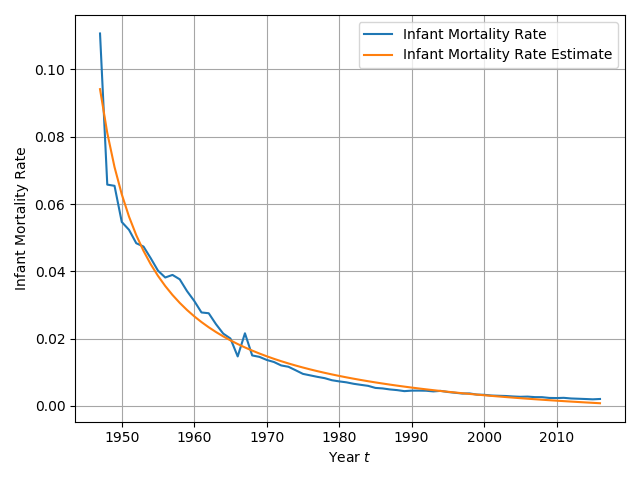
\includegraphics[width=0.50\textwidth]{\FigureDir/mortality/smooth_0/_infant_mortality_rate_predicted.png}
			  \end{tabular}
		   \end{threeparttable}
		}
	 \end{figure}

\end{frame}

\begin{frame}{Full-Dynamic - Mortality}

	Mortality fit to generalized beta 2 distribution (same as fertility):
	\begin{align*}
		&f(x|a, b, p, q) = \frac{ax^{ap-1}}{b^{ap}B(p,q)\left(1 + \left(\frac{x}{b}\right)^a\right)^{p+q}} \\
		&\hspace{5mm} \text{where} \hspace{2mm} x \in [0,\infty); a, b, p, q > 0   
	 \end{align*}

\end{frame}

\begin{frame}{Full-Dynamic - Mortality}

	\centering
	Mortality Generalized Beta 2 Parameter Estimates
	\vspace{-5mm}
	\begin{table}[H]
	\begin{minipage}[t]{0.33\textwidth}
		\begin{figure}[H]
			\begin{subfigure}{\textwidth}
				\centering
				\includegraphics[width=0.85\textwidth]{\FigureDir/mortality/smooth_0/_a_predicted.png}
				\vspace{-3mm}
				\\ \scalebox{0.7}{(a) \(a\)}
			\end{subfigure}

			\begin{subfigure}{\textwidth}
				\centering
				\includegraphics[width=0.85\textwidth]{\FigureDir/mortality/smooth_0/_b_predicted.png}
				\vspace{-3mm}
				\\ \scalebox{0.7}{(b) \(b\)}
			\end{subfigure}
		\end{figure}
	\end{minipage}% <-- this "%" symbol is important
	\begin{minipage}[t]{0.33\textwidth}
		\begin{figure}[H]
			\vspace{10mm}
			\begin{subfigure}{\textwidth}
				\centering
				\includegraphics[width=0.85\textwidth]{\FigureDir/mortality/smooth_0/_p_predicted.png}
				\\ \scalebox{0.7}{(c) \(p\)}
			\end{subfigure}
		\end{figure}
	\end{minipage}% <-- this "%" symbol is important
	\begin{minipage}[t]{0.33\textwidth}
		\begin{figure}[H]
			\begin{subfigure}{\textwidth}
				\centering
				\includegraphics[width=0.85\textwidth]{\FigureDir/mortality/smooth_0/_q_predicted.png}
				\vspace{-3mm}
				\\ \scalebox{0.7}{(d) \(q\)}
			\end{subfigure}

			\begin{subfigure}{\textwidth}
				\centering
				\includegraphics[width=0.85\textwidth]{\FigureDir/mortality/smooth_0/_scale_predicted.png}
				\vspace{-3mm}
				\\ \scalebox{0.7}{(e) Scale}
			\end{subfigure}
		\end{figure}
	\end{minipage}
	\end{table}

\end{frame}

\begin{frame}{Full-Dynamic - Mortality}

	\begin{figure}[H]
		Mortality Generalized Beta 2 Model Fit
		\begin{subfigure}{0.5\textwidth}
			\centering
			\includegraphics[width=0.6\textwidth]{\FigureDir/mortality/smooth_0/_aggregate_true.png}
			\vspace{-5mm}
			\caption{Data}
		\end{subfigure}% <-- this "%" symbol is important
		~ % <-- this "~" symbol is important
		\begin{subfigure}{0.5\textwidth}
			\centering
			\includegraphics[width=0.6\textwidth]{\FigureDir/mortality/smooth_0/_aggregate_predicted.png}
			\vspace{-5mm}
			\caption{Model}
		\end{subfigure}%
		\newline
		\begin{subfigure}{0.5\textwidth}
			\centering
			\includegraphics[width=0.6\textwidth]{\FigureDir/mortality/smooth_0/_aggregate_overlay_predicted.png}
			\vspace{-5mm}
			\caption{Model Overlays Data}
		\end{subfigure}%
		~ % <-- this "~" symbol is important
		\begin{subfigure}{0.5\textwidth}
			\centering
			\includegraphics[width=0.6\textwidth]{\FigureDir/mortality/smooth_0/_2100.png}
			\vspace{-5mm}
			\caption{Model Forecasts}
		\end{subfigure}%
	\end{figure}

\end{frame}

\begin{frame}{Full-Dynamic - Immigration}
	Immigration fit to linear regression, then forecasted out using an exponential of the form:
	\begin{align*}
		f(x|a, b, c, d, p, s, \beta_0, \beta_1) = e^{a(x-s)^2 + b(x-s) + c} + p 
	 \end{align*}
\end{frame}

\begin{frame}{Full-Dynamic - Immigration}

	\begin{figure}[H]
		\small{Immigration Estimated by Linear Regression and Forecasted by Exponential}
		\begin{subfigure}{0.5\textwidth}
			\centering
			\includegraphics[width=0.6\textwidth]{\FigureDir/immigration/smooth_0/_aggregate_true.png}
			\vspace{-5mm}
			\caption{Data}
		\end{subfigure}% <-- this "%" symbol is important
		~ % <-- this "~" symbol is important
		\begin{subfigure}{0.5\textwidth}
			\centering
			\includegraphics[width=0.6\textwidth]{\FigureDir/immigration/smooth_0/_aggregate_predicted.png}
			\vspace{-5mm}
			\caption{Model}
		\end{subfigure}%
		\newline
		\begin{subfigure}{0.5\textwidth}
			\centering
			\includegraphics[width=0.6\textwidth]{\FigureDir/immigration/smooth_0/_aggregate_overlay_predicted.png}
			\vspace{-5mm}
			\caption{Model Overlays Data}
		\end{subfigure}%
		~ % <-- this "~" symbol is important
		\begin{subfigure}{0.5\textwidth}
			\centering
			\includegraphics[width=0.6\textwidth]{\FigureDir/immigration/smooth_0/_2100.png}
			\vspace{-5mm}
			\caption{Model Forecasts}
		\end{subfigure}%
	\end{figure}

\end{frame}

\begin{frame}{Full-Dynamic - Population}

	\begin{figure}[H]
		Population Forecasts, Initial Population Set to 1970
		\begin{subfigure}{0.5\textwidth}
			\centering
			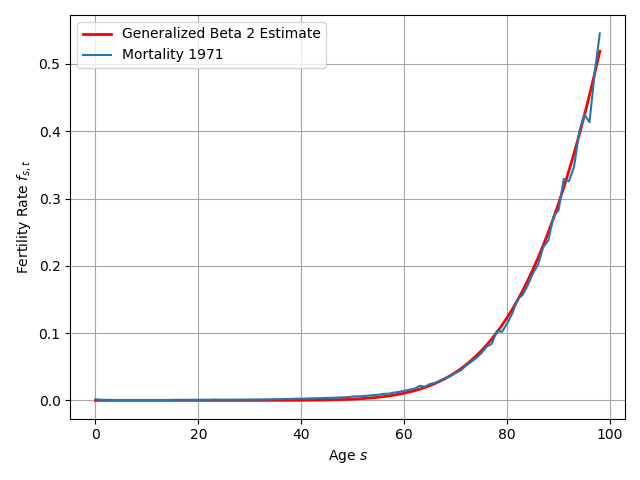
\includegraphics[width=0.6\textwidth]{\FigureDir/population_forecasts/start_1970/1971.png}
			\vspace{-5mm}
			\caption{1971}
		\end{subfigure}% <-- this "%" symbol is important
		~ % <-- this "~" symbol is important
		\begin{subfigure}{0.5\textwidth}
			\centering
			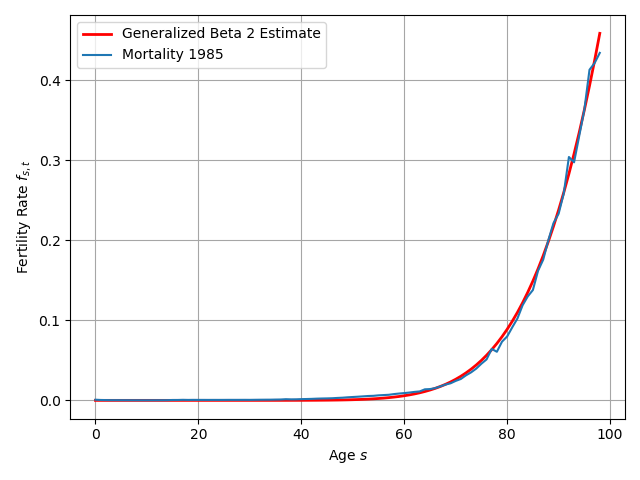
\includegraphics[width=0.6\textwidth]{\FigureDir/population_forecasts/start_1970/1985.png}
			\vspace{-5mm}
			\caption{1985}
		\end{subfigure}%
		\newline
		\begin{subfigure}{0.5\textwidth}
			\centering
			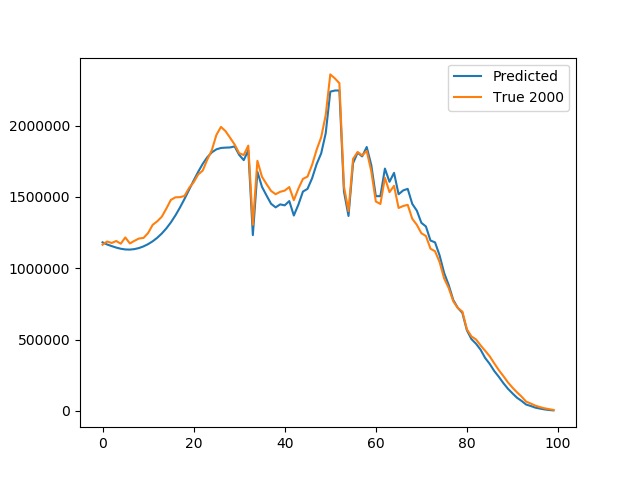
\includegraphics[width=0.6\textwidth]{\FigureDir/population_forecasts/start_1970/2000.png}
			\vspace{-5mm}
			\caption{2000}
		\end{subfigure}%
		~ % <-- this "~" symbol is important
		\begin{subfigure}{0.5\textwidth}
			\centering
			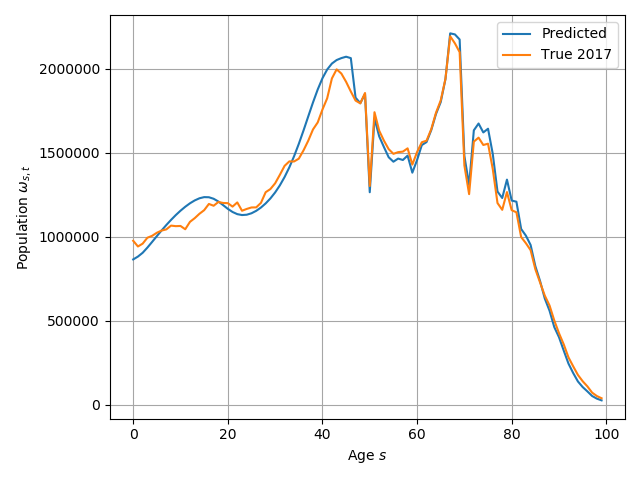
\includegraphics[width=0.6\textwidth]{\FigureDir/population_forecasts/start_1970/2017.png}
			\vspace{-5mm}
			\caption{2017}
		\end{subfigure}%
	\end{figure}

\end{frame}

\begin{frame}{All Models - Steady State Immigration Rates}

	\begin{figure}[H]
		Steady State Immigration Rates
		\begin{subfigure}{0.5\textwidth}
			\centering
			\includegraphics[width=0.6\textwidth]{\DemoDir/static/OrigVsAdjImm.png}
			\vspace{-5mm}
			\caption{Static}
		\end{subfigure}% <-- this "%" symbol is important
		~ % <-- this "~" symbol is important
		\begin{subfigure}{0.5\textwidth}
			\centering
			\includegraphics[width=0.6\textwidth]{\DemoDir/dynamic_full_alternate/OrigVsAdjImm.png}
			\vspace{-5mm}
			\caption{PCA}
		\end{subfigure}%
		\newline
		\begin{subfigure}{0.5\textwidth}
			\centering
			\includegraphics[width=0.6\textwidth]{\DemoDir/dynamic_partial/OrigVsAdjImm.png}
			\vspace{-5mm}
			\caption{Partial-Dynamic}
		\end{subfigure}%
		~ % <-- this "~" symbol is important
		\begin{subfigure}{0.5\textwidth}
			\centering
			\includegraphics[width=0.6\textwidth]{\DemoDir/dynamic_full/OrigVsAdjImm.png}
			\vspace{-5mm}
			\caption{Full-Dynamic}
		\end{subfigure}%
	\end{figure}

\end{frame}

\begin{frame}{All Models - Population Distribution Path}

	\begin{figure}[H]
		Population Distribution Paths
		\begin{subfigure}{0.5\textwidth}
			\centering
			\includegraphics[width=0.6\textwidth]{\DemoDir/static/PopDistPath.png}
			\vspace{-5mm}
			\caption{Static}
		\end{subfigure}% <-- this "%" symbol is important
		~ % <-- this "~" symbol is important
		\begin{subfigure}{0.5\textwidth}
			\centering
			\includegraphics[width=0.6\textwidth]{\DemoDir/dynamic_full_alternate/PopDistPath.png}
			\vspace{-5mm}
			\caption{PCA}
		\end{subfigure}%
		\newline
		\begin{subfigure}{0.5\textwidth}
			\centering
			\includegraphics[width=0.6\textwidth]{\DemoDir/dynamic_partial/PopDistPath.png}
			\vspace{-5mm}
			\caption{Partial-Dynamic}
		\end{subfigure}%
		~ % <-- this "~" symbol is important
		\begin{subfigure}{0.5\textwidth}
			\centering
			\includegraphics[width=0.6\textwidth]{\DemoDir/dynamic_full/PopDistPath.png}
			\vspace{-5mm}
			\caption{Full-Dynamic}
		\end{subfigure}%
	\end{figure}

\end{frame}

\begin{frame}{All Models - Steady State Population Distribution}

	\begin{figure}[H]
		Steady State Population Distributions
		\begin{subfigure}{0.5\textwidth}
			\centering
			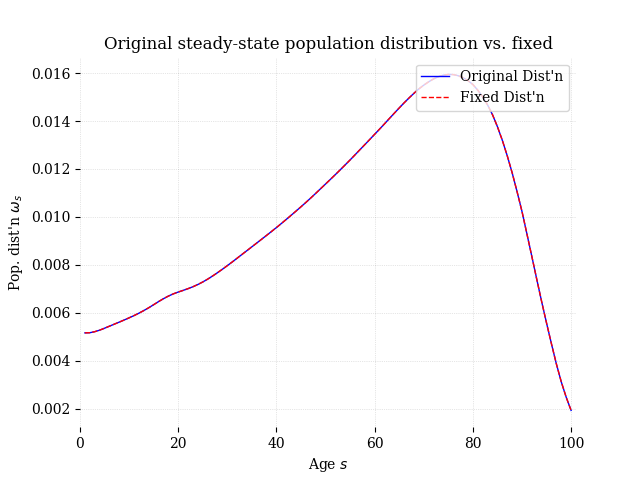
\includegraphics[width=0.6\textwidth]{\DemoDir/static/OrigVsFixSSpop.png}
			\vspace{-5mm}
			\caption{Static}
		\end{subfigure}% <-- this "%" symbol is important
		~ % <-- this "~" symbol is important
		\begin{subfigure}{0.5\textwidth}
			\centering
			\includegraphics[width=0.6\textwidth]{\DemoDir/dynamic_full_alternate/OrigVsFixSSpop.png}
			\vspace{-5mm}
			\caption{PCA}
		\end{subfigure}%
		\newline
		\begin{subfigure}{0.5\textwidth}
			\centering
			\includegraphics[width=0.6\textwidth]{\DemoDir/dynamic_partial/OrigVsFixSSpop.png}
			\vspace{-5mm}
			\caption{Partial-Dynamic}
		\end{subfigure}%
		~ % <-- this "~" symbol is important
		\begin{subfigure}{0.5\textwidth}
			\centering
			\includegraphics[width=0.6\textwidth]{\DemoDir/dynamic_full/OrigVsFixSSpop.png}
			\vspace{-5mm}
			\caption{Full-Dynamic}
		\end{subfigure}%
	\end{figure}

\end{frame}

%===============================================================%
\section{Macroeconomic Model}
%===============================================================%

\begin{frame}{Macroeconomic Model: Short Description}
	\begin{itemize}
		\item Overlapping generations model from Evans (2020)
		\item Households live for 100 periods: 20 periods of youth, outside the labor market; 80 periods of adulthood, contribute to economy
		\item Households choose consumption, labor, and savings to maximize lifetime utility
		\item Households subject to warm bequest motive
		\item Population demographics can evolve over time
		\item Firms choose capital and labor to maximize profits
		\item No government (no taxes or transfers)
	\end{itemize}
\end{frame}

\begin{frame}{Macroeconomic Model: Households}
	Households choose consumption, labor, and savings to maximize
	\begin{dmath*}
		{u(c_{s,t}, n_{s,t}, b_{s+1,t+1}) = \frac{(c_{s,t})^{1-\sigma}-1}{1-\sigma} + e^{g_yt(1-\sigma)}\chi_{n,s}b\left[1-\left(\frac{n_{s,t}}{\tilde{l}}\right)\right]^{\frac{1}{\upsilon}}} \\
		{\hspace{40mm} + \rho_{s,t}\chi_b\frac{(b_{s+1,t+1})^{1-\sigma}-1}{1-\sigma} \hspace{3mm} \forall s,t}
	 \end{dmath*}
	 subject to
	 \begin{gather*}
		c_{s,t} + b_{s+1,t+1} = (1+r_t)b_{s,t} + w_tn_{s,t} + \frac{BQ_t}{\tilde{N}_t} \hspace{3mm} \forall t \hspace{3mm} \text{and} \hspace{3mm} s \geq E \\
		b_{E,t}=b_{E+S,t}=0 \hspace{3mm} \forall t \\
		c_{s,t} \geq 0 \hspace{3mm} \forall s,t
	 \end{gather*}
\end{frame}

\begin{frame}{Macroeconomic Model: Firms}
	Firms have the following Cobb-Douglas production function:
	\begin{equation*}
		Y_t = F(K_t, L_t) \equiv A(K_t)^\alpha(e^{g_yt}L_t)^{1-\alpha} \forall t \hspace{3mm} \alpha \in (0, 1) \hspace{3mm} \text{and} \hspace{3mm} A>0
	\end{equation*}
	Firms then choose capital and labor to maximize profits:
	\begin{equation*}
		PR_t = A(K_t)^\alpha(e^{g_yt}L_t)^{1-\alpha} - (r_t + \delta)K_t - w_tL_t \hspace{3mm} \forall t
	 \end{equation*}
\end{frame}

%===============================================================%
\section{Results}
%===============================================================%

%===============================================================%
\subsection{Steady State}
%===============================================================%

\begin{frame}{Summary of Steady State Results}
	\begin{itemize}
		\item Compared to baseline (static), consumption/savings everywhere higher in dynamic models
		\item PCA results: dramatically more consumption/savings with old population relative to partial- and full-dynamic
		\item Compared to baseline (static), labor everywhere lower in dynamic models
		\item PCA results: more labor for young population, less labor for old population relative to partial- and full-dynamic
	\end{itemize}
\end{frame}

\begin{frame}{Steady State Consumption}

	\begin{figure}[H]
		\begin{subfigure}{0.5\textwidth}
		   \centering
		   \includegraphics[width=\textwidth]{\SSDir/pct_change/images/SS_c_static.png}
		   \caption{Static Demographics}
		\end{subfigure}%
		~
		\begin{subfigure}{0.5\textwidth}
		   \centering
		   \includegraphics[width=\textwidth]{\SSDir/pct_change/images/SS_c.png}
		   \caption{All Other Demographics (\% Deviation from Static)}
		\end{subfigure}
	 \end{figure}

\end{frame}

\begin{frame}{Steady State Savings}

	\begin{figure}[H]
		\begin{subfigure}{0.5\textwidth}
		   \centering
		   \includegraphics[width=\textwidth]{\SSDir/pct_change/images/SS_b_static.png}
		   \caption{Static Demographics}
		\end{subfigure}%
		~
		\begin{subfigure}{0.5\textwidth}
		   \centering
		   \includegraphics[width=\textwidth]{\SSDir/pct_change/images/SS_b.png}
		   \caption{All Other Demographics (\% Deviation from Static)}
		\end{subfigure}
	 \end{figure}

\end{frame}

\begin{frame}{Steady State Labor}

	\begin{figure}[H]
		\begin{subfigure}{0.5\textwidth}
		   \centering
		   \includegraphics[width=\textwidth]{\SSDir/static/images/SS_n.png}
		   \caption{Static Demographics}
		\end{subfigure}%
		~
		\begin{subfigure}{0.5\textwidth}
		   \centering
		   \includegraphics[width=\textwidth]{\SSDir/pct_change/images/SS_n.png}
		   \caption{All Other Demographics (\% Deviation from Static)}
		\end{subfigure}
	 \end{figure}

\end{frame}

%===============================================================%
\subsection{Transition Path}
%===============================================================%

\begin{frame}{Summary of Transition Path Results}
	\begin{itemize}
		\item Transition path results difficult to interpret: difference between baseline (static) and dynamic models too large to explain
	\end{itemize}
\end{frame}

\begin{frame}{Transition Path of Aggregate Output}
	\begin{figure}[H]
		\begin{subfigure}{0.5\textwidth}
		   \centering
		   \includegraphics[width=\textwidth]{\TPDir/static/images/TP_Y_path.png}
		   \caption{Static Demographics}
		\end{subfigure}%
		~
		\begin{subfigure}{0.5\textwidth}
		   \centering
		   \includegraphics[width=\textwidth]{\TPDir/pct_change/images/TP_Y_path.png}
		   \caption{All Other Demographics (\% Deviation from Static)}
		\end{subfigure}
	 \end{figure}
\end{frame}

\begin{frame}{Transition Path of Aggregate Consumption}

	\begin{figure}[H]
		\begin{subfigure}{0.5\textwidth}
		   \centering
		   \includegraphics[width=\textwidth]{\TPDir/static/images/TP_C_path.png}
		   \caption{Static Demographics}
		\end{subfigure}%
		~
		\begin{subfigure}{0.5\textwidth}
		   \centering
		   \includegraphics[width=\textwidth]{\TPDir/pct_change/images/TP_C_path.png}
		   \caption{All Other Demographics (\% Deviation from Static)}
		\end{subfigure}
	 \end{figure}

\end{frame}

\begin{frame}{Transition Path of Aggregate Capital}

	\begin{figure}[H]
		\caption{\label{fig:tp_K_pct}Time Path of Aggregate Capital \(\hat{K}_t\)}
		\begin{subfigure}{0.5\textwidth}
		   \centering
		   \includegraphics[width=\textwidth]{\TPDir/static/images/TP_K_path.png}
		   \caption{Static Demographics}
		\end{subfigure}%
		~
		\begin{subfigure}{0.5\textwidth}
		   \centering
		   \includegraphics[width=\textwidth]{\TPDir/pct_change/images/TP_K_path.png}
		   \caption{All Other Demographics (\% Deviation from Static)}
		\end{subfigure}
	 \end{figure}

\end{frame}

\begin{frame}{Transition Path of Aggregate Labor Supply}

	\begin{figure}[H]
		\begin{subfigure}{0.5\textwidth}
		   \centering
		   \includegraphics[width=\textwidth]{\TPDir/static/images/TP_L_path.png}
		   \caption{Static Demographics}
		\end{subfigure}%
		~
		\begin{subfigure}{0.5\textwidth}
		   \centering
		   \includegraphics[width=\textwidth]{\TPDir/pct_change/images/TP_L_path.png}
		   \caption{All Other Demographics (\% Deviation from Static)}
		\end{subfigure}
	 \end{figure}

\end{frame}

%===============================================================%
\section{Conclusion}
%===============================================================%

\begin{frame}{Conclusion}
	\begin{itemize}
		\item Full dynamic demographic forecasting seems realistic, but forecasts vary depending on model used
		\item Macroeconomic results differ by demographic assumptions
		\begin{itemize}
			\item Distributional differences
			\item Short-run and medium-run aggregate variable differences
		\end{itemize}
		\item Results certainly apply to demographic assumptions used in other models
		\item Extensions: endogenous fertility, in the spirit of Barro and Becker (1989)
	\end{itemize}
\end{frame}

%===============================================================%
\section{Bibliography}
%===============================================================%

\begin{frame}{Bibliography}
	\centering
	\scalebox{0.5}{%
		\vbox{%
			\begin{itemize}
				\item \textbf{Barro, Robert J. and Gary S. Becker}, ``Fertility Choice in a Model of Economic Growth,”\textit{Econometrica}, 1989, pp. 481–501.
				\item \textbf{DeBacker, Jason and Richard W. Evans}, \textit{OG-USA: Documentation for the Large-Scale DynamicGeneral Equilibrium Overlapping Generations Model for U.S. Policy Analysis 2018}.
				\item \textbf{Evans, Richard W.}, \textit{Simple OG Model with Non-constant Demographic Dynamics and Productivity Growth} 2020.
				\item \textbf{Human Fertility Collection}, ``Japan - ASFR and CPFR, Standardized Age Scale,” 2018.  Data retrieved from Max Planck Institute for Demographic Research, \url{https://www.fertilitydata.org/cgi-bin/country.php?code=jpn}.
				\item \textbf{Hyndman, Rob J.}, ``Demography:  Forecasting Mortality, Fertility, Migration and Population Data,” 2019. Package retrieved from \url{https://www.rdocumentation.org/packages/demography/versions/1.22}.
				\item \textbf{-- and Md. Shahid Ullah}, ``Robust Forecasting of Mortality and Fertility Rates:  A Functional DataApproach,” \textit{Computational Statistics \& Data Analysis}, 2007, \textit{51}(10), 4942–4956.
				\item \textbf{Japanese Mortality Database}, ``Births and Deaths,” 2018. Data retrieved from National Institute ofPopulation and Social Security Research,\url{http://www.ipss.go.jp/p-toukei/JMD/index-en.asp}.
			\end{itemize}
		}
	}
\end{frame}

%===============================================================%
\end{document}
%===============================================================% 